%2S -необходимо взять материал из materials/Armeev_disser.pdf пункт 4.5 (со стр 71) небходимо переформулировать так, чтобы не нашел антиплагиат
    
  
  Динамика нуклеосом может активно регулироваться взаимодействиями с различными белками. Нашими коллегами был произведен ряд экспериментов методом spFRET для изучения конформационных перестроек в нуклеосомах при его взаимодействии с комплексом шаперонов FACT. В ходе эксперимента был введен ряд пар меток (Cy3-Cy5) разные положения нуклеосомной ДНК: проксимальные метоки - вблизи входа в нуклеосому, медиальные - по центру нуклеосомы и дистальные - вблизи выхода из нуклеосомы (Рис. \ref{fig:p6_3_f22}). По изменению сигнала spFRET было обнаружено, что связывание FACT вызывает существенные, но обратимые изменения в сигнале FRET. С использованием этих данных методами интегративного моделирования нами были построены модели возможных конформационных перестроек в нуклеосомах.
    
\begin{figure} [H]
    \centering
    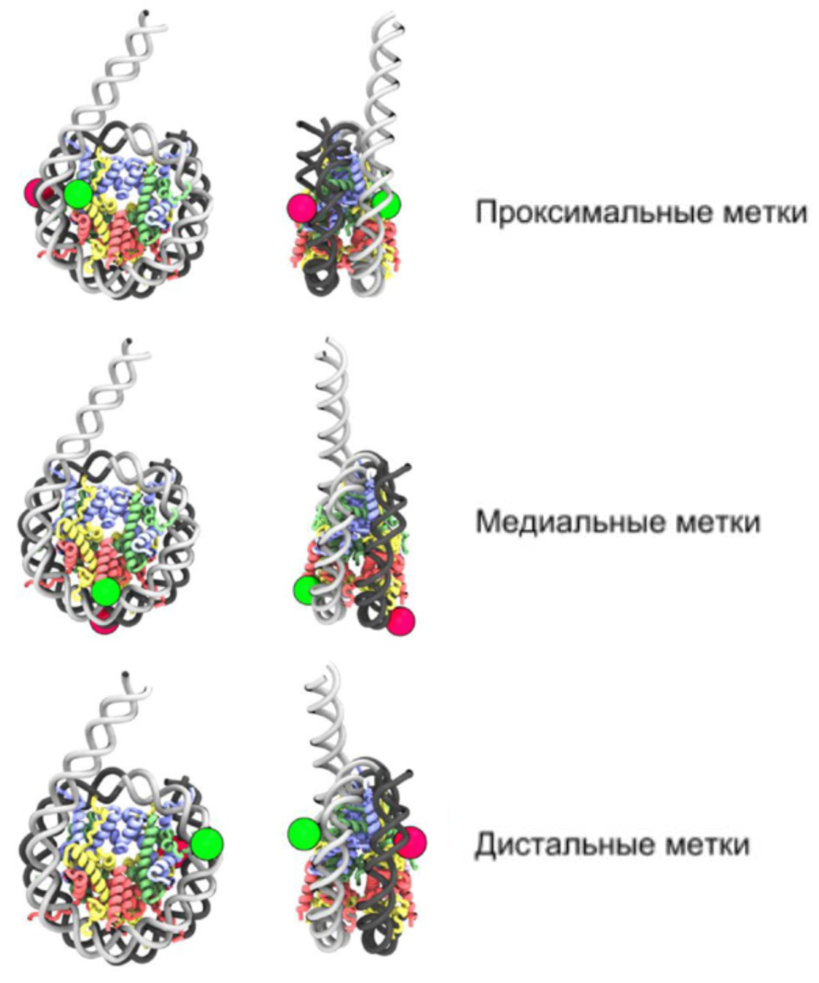
\includegraphics[width=\textwidth]{images/p6/p6_3/p6_3_f22.pdf}
    \caption[Расположение флуоресцентных меток на нуклеосоме в spFRET экспериментах]{Расположение флуоресцентных меток на нуклеосоме в spFRET экспериментах. Зеленым показаны положения донора (Cy3), красным - акцептора (Cy5).}
    \label{fig:p6_3_f22}
\end{figure}
    
    
    
    На основе измерений, в том числе с использованием измерения фактора детекции (см. главу \ref{part1_1_md}), нами был сконструирован и отобран ряд возможных моделей, которые согласуются с экспериментальными данными. Установлено, что для  значительного изменения эффективности переноса, наблюдаемого в эксперименте, величина откручивания ДНК от нуклеосомы должна составлять около 100 н.п. ДНК, при этом около 40 н.п. должно откручивать с одной стороны и около 60 н.п. с другой стороны (рис. \ref{fig:p6_3_f23}).
    
\begin{figure} [H]
    \centering
    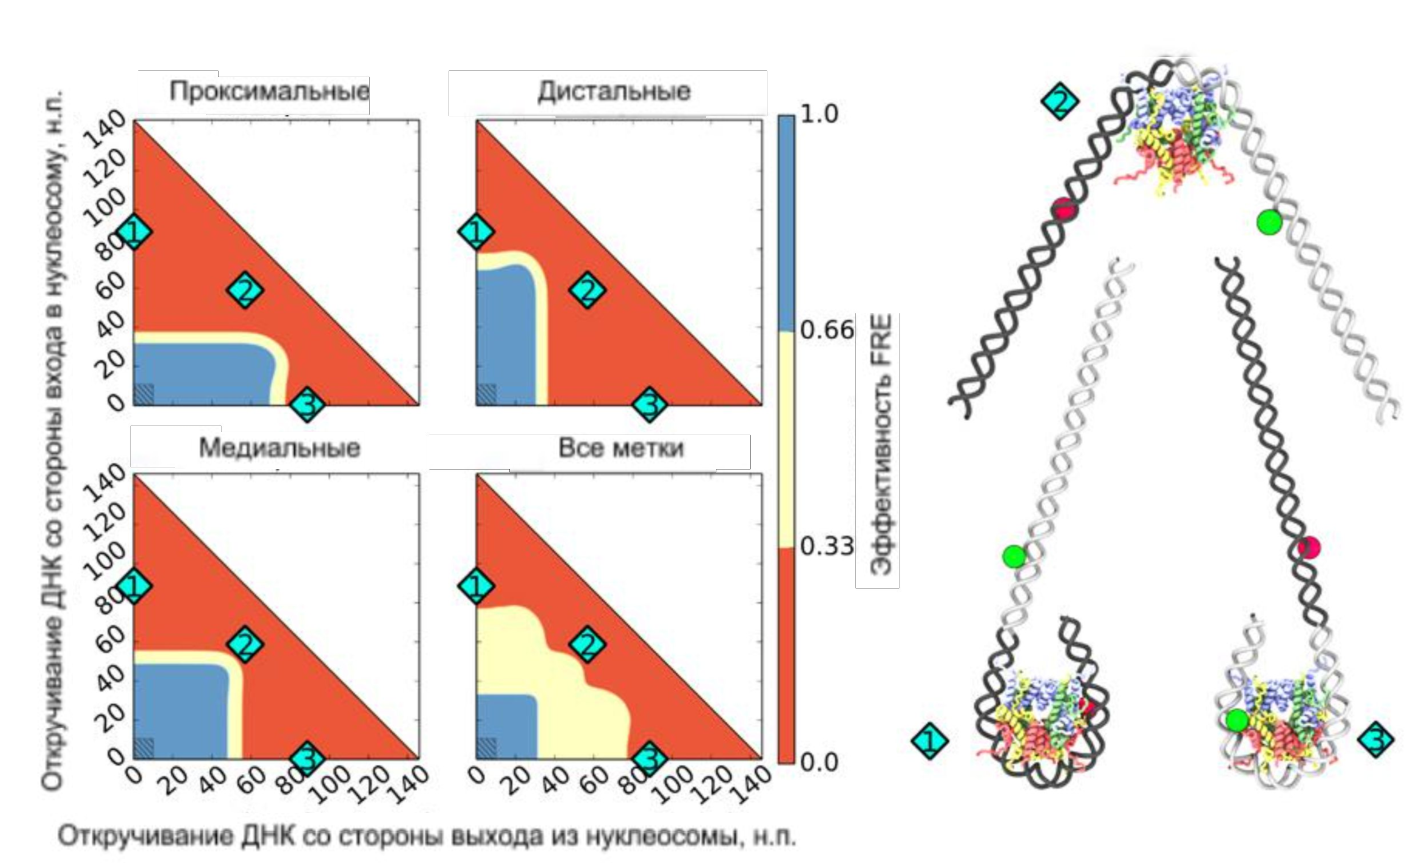
\includegraphics[width=\textwidth]{images/p6/p6_3/p6_3_f23.pdf}
    \caption[Анализ зависимости эффективности FRET от степени разворачивания нуклеосом]{Анализ зависимости эффективности FRET от степени разворачивания нуклеосом. Слева: тепловые карты ожидаемых эффективностей переноса энергии на трех парах флуорофоров. Красные и голубые области соответствуют степеням откручивания ДНК с низкой и высокой эффективностью FRET соответственно. Затемненные участки тепловых карт (левый нижний угол) отвечают нативным состояниям нуклеосом (состояниям близким к наблюдаемым в кристаллических структурах). Справа: Модели конформаций нуклеосом, соответствующие отмеченным номерам на картах.}
    \label{fig:p6_3_f23}
\end{figure}
    
    По этим данным были построены молекулярные модели, соответствующие таким степеням отворота ДНК (Рис. \ref{fig:p6_3_f24}): модель откручивания ДНК с сохранением гистонового октамера (Рис. \ref{fig:p6_3_f24}), модель откручивания ДНК с образованием структуры ``бабочка'' (Рис. \ref{fig:p6_3_f24}3) , модель с образованием двух хемисом (Рис. \ref{fig:p6_3_f24}5), а также модель полного разрушения октамера гистонов (Рис. \ref{fig:p6_3_f24}). Все эти модели в равной степени соответствуют наблюдаемым изменениям в эффективности переноса энергии в присутствии гистонового шаперона FACT.
    
\begin{figure} [H]
    \centering
    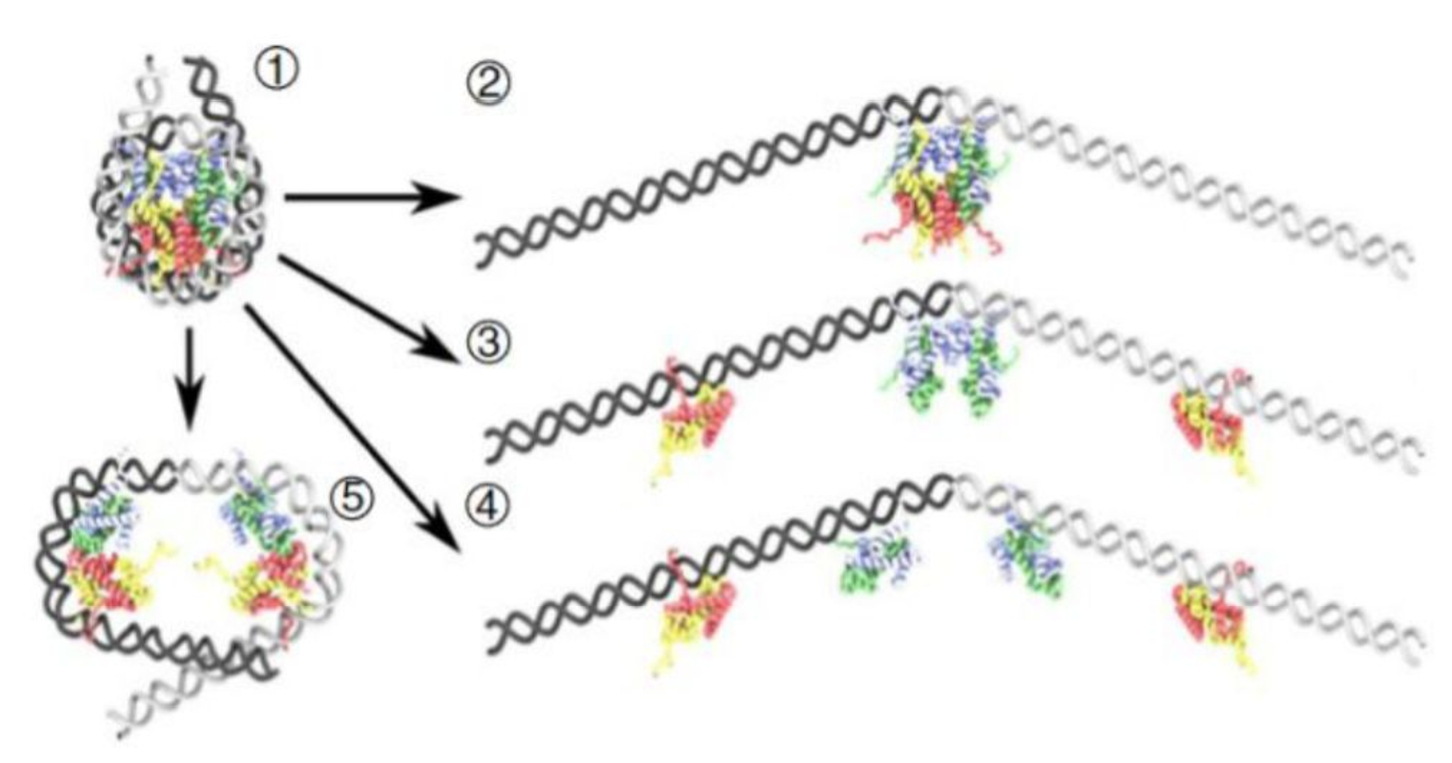
\includegraphics[width=\textwidth]{images/p6/p6_3/p6_3_f24.pdf}
    \caption[Модели разворачивания нуклеосом, вызванного взаимодействием с шапероном FACT]{Модели разворачивания нуклеосом, вызванного взаимодействием с шапероном FACT. Интактные нуклеосомы (1) могут разворачиваться от интактного октамера (2), ДНК может отворачиваться с разрушением (3) или без (4) разрушения интерфейса взаимодействия гистонов H3–H3 или путем открытия интерфейса H3-H3 без откручивания ДНК (5) с формированием двух хемисом.}
    \label{fig:p6_3_f24}
\end{figure}
    
    Потеря гистонов в процессе откручивания ДНК при низких концентрациях нуклеосом должна быть необратимой, так как в ходе экспериментов в раствор дополнительно добавляли конкурирующую за гистоны ДНК, не меченную флуорофорами. Тот факт, что наблюдаемый эффект был обратим, свидетельствует о том, что разворачивание октамера должно происходить без потери гистонов H2A-H2B.
    
    
    
    
    
    
    
    
    
    
    
    
    
    
    
    
    
    
    
    
    
    
    
    
    
    
    
    
    
    
    
    
    
    
    
    
    
    
    
    
    
    
    
    
    
    
    
    
    
    
    
    
    
    
    
    
    
    
    
    
    
    